\entry{Semana del 02/06/2025}
Ya están completamente diseñadas las placas, tanto con las borneras de 2 pines a PCB, de ELEMON, como con los jacks BNC-PCB de 90° de iUrbaNet. 

\section{PCB con Borneras.}
\begin{figure}[!ht]
	\begin{minipage}[c]{0.3325\textwidth}
			\begin{subfigure}{\textwidth}
					\centering
					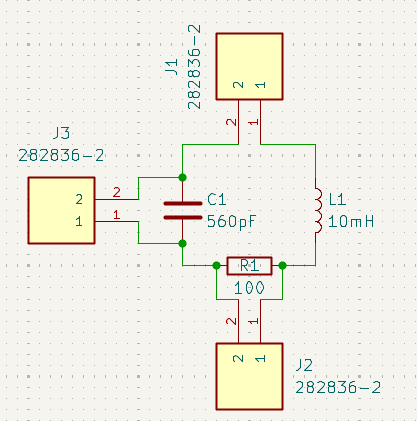
\includegraphics[width=0.978\textwidth]{Figures/02_06_2025/Schematic_borneras}
					\captionsetup{width=0.8\textwidth}
					\subcaption{}
				\end{subfigure}
		\end{minipage}\begin{minipage}[c]{0.332149\textwidth}
			\begin{subfigure}{\textwidth}
					\centering
					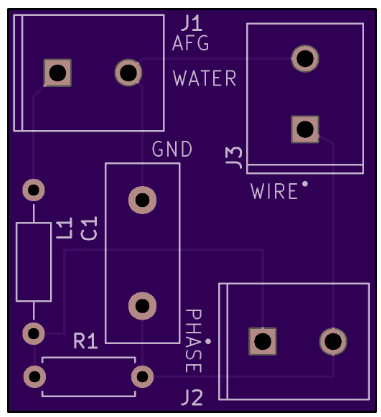
\includegraphics[width=0.978\textwidth]{Figures/02_06_2025/PCB_Top_borneras.png}
					\captionsetup{width=0.8\textwidth}
					\subcaption{}
				\end{subfigure}
		\end{minipage}\begin{minipage}[c]{0.3321249\textwidth}
		\begin{subfigure}{\textwidth}
			\centering
			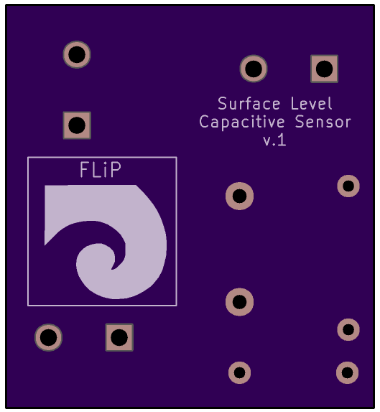
\includegraphics[width=0.978\textwidth]{Figures/02_06_2025/PCB_Bottom_borneras}
			\captionsetup{width=0.8\textwidth}
			\subcaption{}
		\end{subfigure}
	\end{minipage}
	\caption{A la izquierda el esquema del circuito eléctrico que corresponde a la placa. A la derecha la vista superior e inferior de la placa terminada.} %  y  
	\label{fig:}
\end{figure}




\begin{figure}[!ht]
	\begin{minipage}[c]{0.5\textwidth}
			\begin{subfigure}{\textwidth}
					\centering
					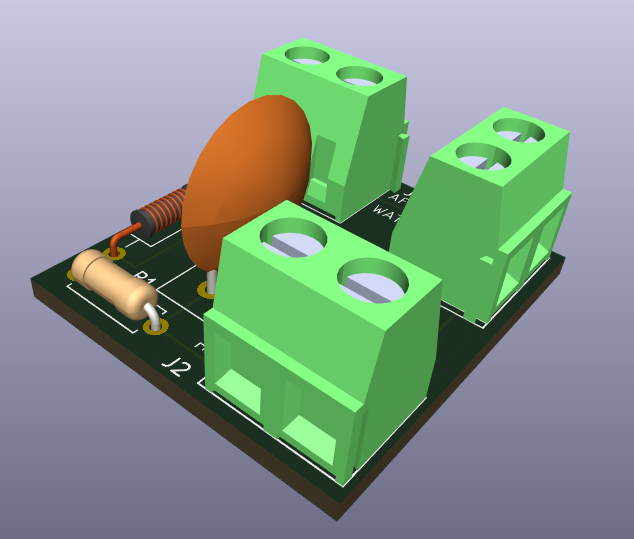
\includegraphics[width=0.82\textwidth]{Figures/02_06_2025/PCB_3D_perfil_borneras1}
					\captionsetup{width=0.8\textwidth}
					\subcaption{}
				\end{subfigure}
		\end{minipage}\begin{minipage}[c]{0.49\textwidth}
			\begin{subfigure}{\textwidth}
					\centering
					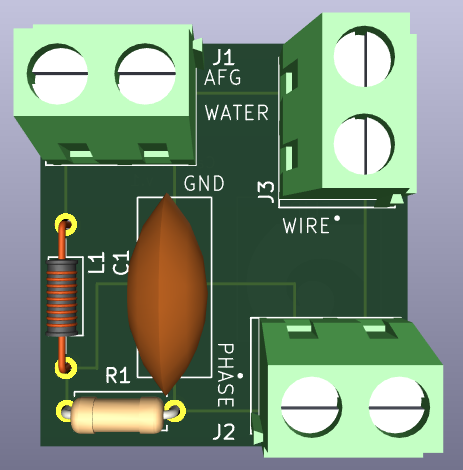
\includegraphics[width=0.78\textwidth]{Figures/02_06_2025/PCB_3D_top_borneras}
					\captionsetup{width=0.8\textwidth}
					\subcaption{}
				\end{subfigure}
		\end{minipage}
	\caption{}
	\label{fig:}
\end{figure}



We detected a 2 layer board of 1.02 x 1.12 inches (26.0 x 28.5mm)
3 boards will cost 5.70 % $ $ 

% 5 Figures/02_06_2025/PCB_Bottom_borneras
% Figures/02_06_2025/PCB_Top_BNC

\section{PCB con BNC.}
\begin{figure}[!ht]
	\begin{minipage}[c]{0.3325\textwidth}
		\begin{subfigure}{\textwidth}
			\centering
			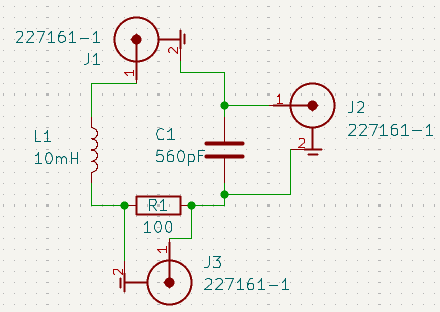
\includegraphics[width=0.978\textwidth]{Figures/02_06_2025/Schematic_BNC}
			\captionsetup{width=0.8\textwidth}
			\subcaption{}
		\end{subfigure}
	\end{minipage}\begin{minipage}[c]{0.332149\textwidth}
		\begin{subfigure}{\textwidth}
			\centering
			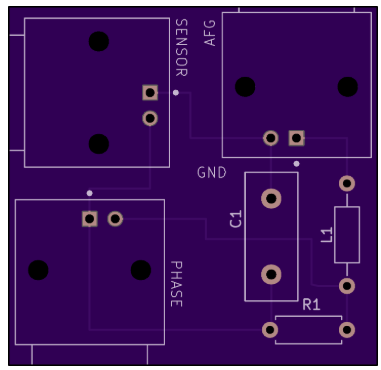
\includegraphics[width=0.978\textwidth]{Figures/02_06_2025/PCB_Top_BNC.png}
			\captionsetup{width=0.78\textwidth}
			\subcaption{}
		\end{subfigure}
	\end{minipage}\begin{minipage}[c]{0.3321249\textwidth}
		\begin{subfigure}{\textwidth}
			\centering
			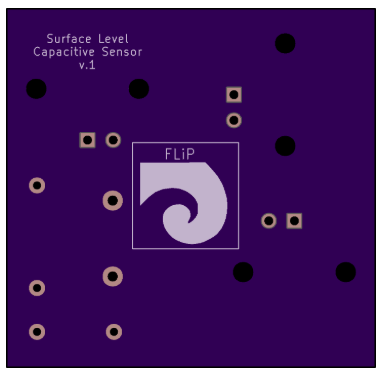
\includegraphics[width=0.978\textwidth]{Figures/02_06_2025/PCB_Bottom_BNC}
			\captionsetup{width=0.8\textwidth}
			\subcaption{}
		\end{subfigure}
	\end{minipage}
	\caption{A la izquierda el esquema del circuito eléctrico que corresponde a la placa. A la derecha la vista superior e inferior de la placa terminada.}
	\label{fig:}
\end{figure}





\begin{figure}[!ht]
	\begin{minipage}[c]{0.5\textwidth}
		\begin{subfigure}{\textwidth}
			\centering
			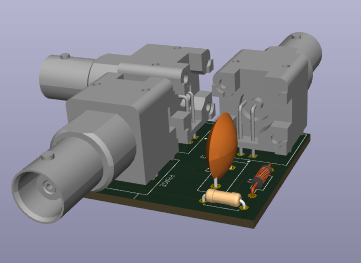
\includegraphics[width=0.98\textwidth]{Figures/02_06_2025/PCB_3D_perfil_BNC}
			\captionsetup{width=0.8\textwidth}
			\subcaption{}
		\end{subfigure}
	\end{minipage}\begin{minipage}[c]{0.49\textwidth}
		\begin{subfigure}{\textwidth}
			\centering
			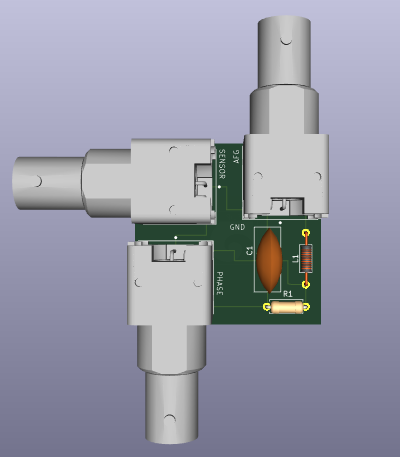
\includegraphics[width=0.8\textwidth,angle=90,origin=c]{Figures/02_06_2025/PCB_3D_top_BNC}
			\captionsetup{width=0.8\textwidth}
			\subcaption{}
		\end{subfigure}
	\end{minipage}
	\caption{}
	\label{fig:}
\end{figure}



We detected a 2 layer board of 1.44 x 1.40 inches (36.5 x 35.5mm)
3 boards will cost 10.05 % $ $



